%!TEX root = ../main.tex
\chapter{Design and Methodology}\label{ch:methodology}
%There are two main requirements to build a dependency graph and critical path analysis testbed. 
%First, we require tools to perform critical path analysis on mobile page loads, to determine the bottlenecks. Second, we need to design an experimental testbed that will allow us to perform comparison studies in the presence of large variances.
To overcome challenges addressed in \S\ref{ch:introduction}, we design and build our own testbed.
To address {\em dependency} challenges, we use WProf \cite{wprof} which takes into account internal page dependencies and to address high {\em variances} in a page load process, we provide a controlled environment to run our experiments.
\section{WProf}
WProf is a tool built atop the open source Chromium browser and is able to infer dependency policies of the browser. 
WProf uses fine-grained timing of activities involved in a page load process to accurately extract the page {\em dependency graph} and the {\em critical path} inside such graph.
We say an activity $a_2$ is dependent on a previously scheduled activity $a_1$ , if $a_2$ can be executed only after $a_1$ is being executed or completed. \\
Considering activities as nodes of a graph  and inter-dependency relations as the edges of such graph, the resulting graph would be a DAG (Directed Acyclic Graph) which we call {\em dependency graph} hereafter.\\

\noindent {\em Critical path} is the sequence of activities which add up to the longest overall duration inside the dependency graph.\\

\section{WProf-M} To perform critical path analysis on mobile devices, we use a version of WProf on Android Chromium Version 31.0.1626.0. As a first step, we repeat our browser instrumentation experiments on mobile browsers to infer the dependency policies on the Android Chromium browser. To infer dependency policies in networking loading and computational activities, we load carefully crafted test pages. The set of Web pages we use to infer the dependency policies can be found at \url{wprof.cs.washington.edu/tests/}. \\

\noindent Next, we instrument the Android Chromium browser to record the timings of each page load activity and use the timing and the dependency policy to extract the dependency graph and compute the critical path.

\section{Testbed Design} One of the challenges in studying effect of an optimization on page load time is that Web page loads have high variance~\cite{spdy_nsdi}. The variance makes it non-trivial to isolate the performance of the mobile browser: if the page load times on the mobile browser is very different when an optimization is applied, the difference could be because of the optimization or because of page load variance.

\noindent We design an experimental testbed that minimizes variance when loading pages before and after optimizations. We make the following design choices:
 \begin{itemize}
  \item  We serve pages from the local server. To this end, we download the entire page locally on the server and convert all the external links to local links.  This minimizes variances caused by changes to the page. 
   \item When comparing mobile and desktop browsers, we load the same page on the mobile and the desktop browser, rather than loading the mobile version of the page (or {\em mpages}) to perform more direct comparisons.
    \item  We emulate different network conditions using a traffic controller to ensure that both the mobile and the desktop browser load pages under the same network conditions.
    \end{itemize}

\noindent To ensure that the results we get from our controlled setting applies more broadly, we perform additional experiments where the three restrictions are removed; i.e., we load pages directly from the Web server, we load {\em mpages}, and we use real networks. Our additional experiments show that the conclusions we derive from our controlled experiments also apply more generally. \\

 \begin{figure}[!htb]
  \centering
    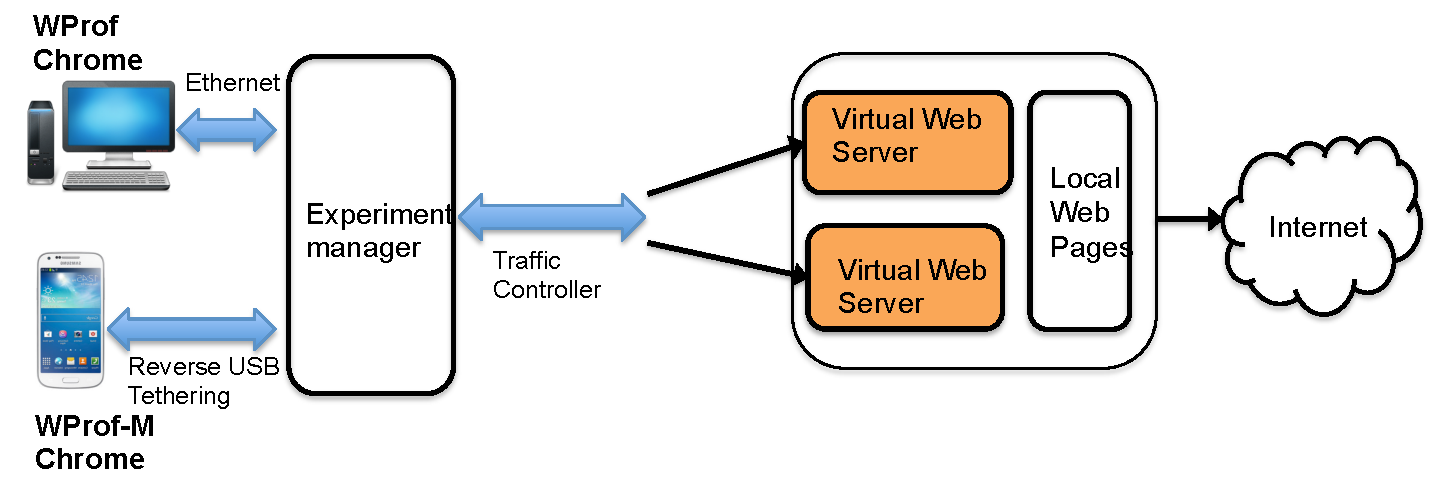
\includegraphics[width=0.9 \textwidth]{./figures/methodology/architecture.pdf}
  \caption{Testbed architecture}
  \label{fig:architecture}
\end{figure}

\noindent Figure~\ref{fig:architecture} shows our experimental testbed. At the client side, we load Web pages on a phone running Android Chromium instrumented with WProf-M, and on a desktop running WProf instrumented Chromium. All Web page loads go through the experiment manager. The manager stores logs generated by WProf and WProf-M and configures the traffic controller and the Web server if needed.  We use USB tethering to connect the mobile device to the experiment manager rather than connect using WiFi because we observed large variances in WiFi latencies.\\

\noindent On the server side, we leverage virtual machines to run multiple web servers on the same platform. To isolate the different network stacks for the difference virtual servers, we use Linux network namespace~\cite{namespace}, similar to \cite{mahimahi}.  To emulate different network conditions, we are using  Linux Traffic Control (TC). Before each experiment, we run ping and iperf tools to test that the emulated network has the expected bandwidth and delay values. 

\section{Parameters}
\label{sec:parameters}

The parameters used in our testbed are as follow\\

{\noindent {\bf Server and Client:}} All Linux instances are virtual machines running inside a VMware ESXi 6.0  Bare-Metal Hypervisor. On average, 4 cores at 2.6GHz and 2GB of RAM has been assigned to each virtual machine. \\

\noindent We use two Samsung Galaxy S4 phones running Android KitKat and Samsung Galaxy S6 phones running Android Lollipop. 
By default, we present experiments conducted on Samsung Galaxy S4 phones on the controlled testbed. \\

{\noindent {\bf Network:}} We run the emulated network experiments on 6 different network profiles under the following bandwidth: 1Mbps, 5Mbps and 20Mbps. We experiment with two round trip delays: 50ms and 150 ms. We inject up to 2\% packet loss rate based on real world studies~\cite{dukkipati_imc2011}.\\
   
 \begin{table}[!htb]
\centering

\begin{tabular}{|l|l|l|l|}
\hline
\rowcolor[HTML]{656565} 
{\color[HTML]{FFFFFF} {\bf }} & {\color[HTML]{FFFFFF} {\bf lab\_WiFi}} & {\color[HTML]{FFFFFF} {\bf lab\_3G}} & {\color[HTML]{FFFFFF} {\bf lab\_4G}} \\ \hline
Average                               & b20-d50                                  & b1-d50                                  & b5-d50                                  \\ \hline
Poor                                     & b20-d150                                  & b1-d150                                  & b5-d150                               \\ \hline
\end{tabular}
\caption{Different network profiles set up in testbed. b: bandwidth in each direction, d: round-trip delay time}
\label{table:net_profiles}
\end{table}

\noindent Table \ref{table:net_profiles} shows the different network profiles. Based on our lab experiments we categorize each pair of bandwidth and round trip delays as latencies seen in WiFi, 3G, and 4G networks.\\
   
{\noindent {\bf Webpages:}} We experiment with 200 Web pages. We randomly choose 40\% of the Web pages from the top 200 websites in Alexa~\cite{alexa}, 30\% from the pages from the bottom of Alexa's 1 million web sites, and the remaining 30\% from news websites on Alexa. We choose a mix of Web pages for the following reason: typically the popular top 200 Web pages on Alexa are smaller (for example, google.com) and are highly optimized. The performance of such Web pages may not be typical. Instead, we include unpopular pages in our mix because they are likely to not be  optimized.  We also choose news websites because they tend to be complex pages. \\

\noindent In the common case, we load the original page on both desktop and mobile. We  perform addition experiments where we load mobile version of the page, that we call {\em mpage}. For example,  \url{m.cnn.com} is an mpage, where the original page is \url{www.cnn.com}. Note that by default, mobile browsers always redirect to the {\em mpage}. We modify the user agent field to force the mobile browser to load the original page. We do this  to directly compare the performance differences between  mobile and desktop browsers.\\

{\noindent {\bf Metrics:}}

\noindent We measure page load  performance using the Page Load Time (PLT) metric. The Page Load Time metric is commonly defined as the time between when the page is requested and when the {\em DOMLoad} event is fired~\cite{wprof}. The DOMLoad event is fired when all  objects are
fetched, processed, and added to the DOM. There has been several alternate metrics to define page load performance such as the above-the-fold metric~\cite{aft}. However, these alternate metrics are not easy to compute and are not yet widely used. \\

\noindent For each page load, we  estimate the critical path. We divide the critical path into the following components:
\begin{itemize}
\item Computation: We sum the time taken by the following activities on the critical path: HTML Parsing, Javascript/CSS evaluation, and rendering. We call this the computational component of the critical path. 
\item Network: We sum the time taken to load each object on the critical path. 
\end{itemize}


